\PassOptionsToPackage{unicode=true}{hyperref} % options for packages loaded elsewhere
\PassOptionsToPackage{hyphens}{url}
%
\documentclass[
]{article}
\usepackage{lmodern}
\usepackage{amssymb,amsmath}
\usepackage{ifxetex,ifluatex}
\ifnum 0\ifxetex 1\fi\ifluatex 1\fi=0 % if pdftex
  \usepackage[T1]{fontenc}
  \usepackage[utf8]{inputenc}
  \usepackage{textcomp} % provides euro and other symbols
\else % if luatex or xelatex
  \usepackage{unicode-math}
  \defaultfontfeatures{Scale=MatchLowercase}
  \defaultfontfeatures[\rmfamily]{Ligatures=TeX,Scale=1}
\fi
% use upquote if available, for straight quotes in verbatim environments
\IfFileExists{upquote.sty}{\usepackage{upquote}}{}
\IfFileExists{microtype.sty}{% use microtype if available
  \usepackage[]{microtype}
  \UseMicrotypeSet[protrusion]{basicmath} % disable protrusion for tt fonts
}{}
\makeatletter
\@ifundefined{KOMAClassName}{% if non-KOMA class
  \IfFileExists{parskip.sty}{%
    \usepackage{parskip}
  }{% else
    \setlength{\parindent}{0pt}
    \setlength{\parskip}{6pt plus 2pt minus 1pt}}
}{% if KOMA class
  \KOMAoptions{parskip=half}}
\makeatother
\usepackage{xcolor}
\IfFileExists{xurl.sty}{\usepackage{xurl}}{} % add URL line breaks if available
\IfFileExists{bookmark.sty}{\usepackage{bookmark}}{\usepackage{hyperref}}
\hypersetup{
  pdftitle={Analyses of 27 years of stand structure development and basal area growth response to a range of initial basal area density levels, 1992-2019},
  pdfauthor={Michael Jull and Hardy Griesbauer},
  pdfborder={0 0 0},
  breaklinks=true}
\urlstyle{same}  % don't use monospace font for urls
\usepackage[margin=1in]{geometry}
\usepackage{longtable,booktabs}
% Allow footnotes in longtable head/foot
\IfFileExists{footnotehyper.sty}{\usepackage{footnotehyper}}{\usepackage{footnote}}
\makesavenoteenv{longtable}
\usepackage{graphicx,grffile}
\makeatletter
\def\maxwidth{\ifdim\Gin@nat@width>\linewidth\linewidth\else\Gin@nat@width\fi}
\def\maxheight{\ifdim\Gin@nat@height>\textheight\textheight\else\Gin@nat@height\fi}
\makeatother
% Scale images if necessary, so that they will not overflow the page
% margins by default, and it is still possible to overwrite the defaults
% using explicit options in \includegraphics[width, height, ...]{}
\setkeys{Gin}{width=\maxwidth,height=\maxheight,keepaspectratio}
\setlength{\emergencystretch}{3em}  % prevent overfull lines
\providecommand{\tightlist}{%
  \setlength{\itemsep}{0pt}\setlength{\parskip}{0pt}}
\setcounter{secnumdepth}{5}
% Redefines (sub)paragraphs to behave more like sections
\ifx\paragraph\undefined\else
  \let\oldparagraph\paragraph
  \renewcommand{\paragraph}[1]{\oldparagraph{#1}\mbox{}}
\fi
\ifx\subparagraph\undefined\else
  \let\oldsubparagraph\subparagraph
  \renewcommand{\subparagraph}[1]{\oldsubparagraph{#1}\mbox{}}
\fi

% set default figure placement to htbp
\makeatletter
\def\fps@figure{htbp}
\makeatother


\title{Analyses of 27 years of stand structure development and basal area growth response to a range of initial basal area density levels, 1992-2019}
\author{Michael Jull and Hardy Griesbauer}
\date{2020-12-01}

\begin{document}
\maketitle

{
\setcounter{tocdepth}{2}
\tableofcontents
}
\hypertarget{internal-text}{%
\section{Internal text}\label{internal-text}}

documentclass: book
output:
bookdown::gitbook:
config:
toc:
collapse: none

\hypertarget{preamble}{%
\section{Preamble}\label{preamble}}

I've organized our manuscript into the sections as outlined on the table of contents on the left side of the screen. A few notes:

\begin{itemize}
\tightlist
\item
  There are a lot of figures and data. To review this manuscript, it might be easiest to use the links on the left to navigate through the sections.
\item
  You will see that some of the figures are labelled ``figure'' or ``appendix'', depending on where I think they might end up in the final manuscript. Easy to change this though!
\end{itemize}

\hypertarget{main-results-and-conclusions-to-focus-on}{%
\subsection{Main results and conclusions to focus on}\label{main-results-and-conclusions-to-focus-on}}

\emph{From a previous e-mail thread:}
3 main elements: (a) influence of residual BA on stand and tree level response, (b) the fact that this is a long-term (27-year) dataset of stand response in a randomized and replicated set of treatments - i.e.~- not ad hoc and not retropective - and (c) the species question - response of subalpine fir and spruce. Further, it is a relatively unique trial for this kind of forest type, asking core questions about stand response.

\hypertarget{to-do-list}{%
\subsection{To-Do list}\label{to-do-list}}

\begin{itemize}
\tightlist
\item
  Finalize the title. Based on previous discussions, the title should refer to: (i) spruce-fir forests, (ii) basal area or growth response to basal area treatments, and (iii) this is an unven-aged stand. Does the title ``Analyses of 27-year growth and stand development responses to partial harvest in an uneven-aged spruce-fir stand'' get close?
\item
  How to refer to treatment units? For some reason, I like the idea of referring to ``high-removal'', ``low-removal'', but we also discussed ``high residual basal area (high RBA)'' and ``low residual basal area (low RBA)''. Once we decide on this, it will be easy to make changes throughout the document.
\item
  Start to whittle down figures/tables
\end{itemize}

\hypertarget{methods}{%
\section{Methods}\label{methods}}

This section will describe the methods we used for data analyses, not field data collection.

From our technical report submitted to FCI earlier:

Our data analyses and summaries examined the effects of the different levels of stand-level basal area density treatments on three main attributes of stand development following treatment. These include, in order:

\begin{enumerate}
\def\labelenumi{\arabic{enumi}.}
\tightlist
\item
  Post-treatment stand basal area dynamics, including the rate and pattern of basal area re-growth and recovery over time following different levels of initial basal area density reductions;
\item
  Stand structural outcomes, including treatment influences on the overall abundance of trees (in sph) by diameter class, within the different treatment types, and;
\item
  Tree species composition outcomes, including treatment influences on the relative abundance and size class distributions of subalpine fir and hybrid white spruce within the different treatment types.
\end{enumerate}

Analyses are grouped into three main categories (below). These are treated as separate categories in the Results section.

\begin{enumerate}
\def\labelenumi{\arabic{enumi}.}
\tightlist
\item
  Tree-level responses to treatment;
\item
  Stand-level responses to treatment:
\end{enumerate}

\hypertarget{tree-level-growth-responses}{%
\subsection{Tree-level growth responses}\label{tree-level-growth-responses}}

To test the hypothesis that tree-level radial growth response over the 1992-2019 period varied with interactions between (i) tree diameter at the time of treatment (1992); (ii) treatment; and (iii) species, we fit linear mixed effects models with log-transformed 1992-2019 diameter increment as the response variable, and treatment, species and log-transformed 1992 diameter as interacting fixed effects, and plot as a random intercept effect. We also fit a similar model with the 1992-2019 diameter increment expressed as a percentage of 1992 diameter. Plots of residuals and fit lines with orginal data were examined to evaluate model goodness of fit. Variance explained for each model are reported using the approach described in Nakagawa et al.~{[}-@Nakagawa2013{]}, as implemented in the MuMIn package for R {[}@add later{]}.

\hypertarget{stand-level-growth-and-structure}{%
\subsection{Stand-level growth and structure}\label{stand-level-growth-and-structure}}

\hypertarget{stand-level-volume-and-basal-area-estimates}{%
\subsubsection{Stand-level volume and basal area estimates}\label{stand-level-volume-and-basal-area-estimates}}

Total and merchantable volumes were estimated for trees using species- and region-specific equations {[}@nigh2016{]} based on tree height and DBH. Consistent with forest management practices in British Columbia, we estimated volumes for trees meeting a minimum diameter utilization limit of 17.5cm DBH. For trees lacking a tree height measurement, we estimated height by fitting a single diameter-height model developed with a linear mixed effects model, with log-transformed DBH as a fixed effect, and tree nested within plot as a random effect. Trees with broken tops were omitted from diameter-height models. We summed tree-level estimates of volume and basal area to generate stand-level estimates for each plot. To test the hypothesis that changes in stand attributes over 27 years varied by treatment, we fit separate linear models with stand total volume, basal area, and density as response variables, and the interaction between treatment and year as the independent variable.

\begin{center}\rule{0.5\linewidth}{0.5pt}\end{center}

Appendix 1: Number of growing seasons between each measurement period
\includegraphics[width=3.08in,height=1.75in,keepaspectratio]{_main_files/figure-latex/show paiTable-1.png}

\begin{center}\rule{0.5\linewidth}{0.5pt}\end{center}

\hypertarget{results}{%
\section{Results}\label{results}}

\hypertarget{tree-level}{%
\subsection{Tree-level}\label{tree-level}}

\hypertarget{basal-area-increment-from-1992-2019}{%
\subsubsection{Basal area increment from 1992-2019}\label{basal-area-increment-from-1992-2019}}

The tree-level basal area increment model indicated that interactions between log-transformed tree size, species and treatment explained 47.8\% (marginal R²) of the variation in tree log-transformed 1992-2019 BAI (Table 1). Estimated marginal means from the model showed that between species and among treatments, larger trees increased basal area more than smaller trees (Figure 5). Species contrasts showed that spruce trees increased basal area more than than fir in the high-removal treatment unit, whereas basal growth between the two species was close to equal in the low-removal and control units (Appendix 6). Within each species, treatment contrasts showed that spruce basal area increment in the high-removal unit exceeded spruce growth in both other units (Appendix 7), whereas fir basal area increment in the high- and low-removal units was higher than the control unit, and there were no significant differences between the two harvested units (Appendix 7).

\begin{center}\rule{0.5\linewidth}{0.5pt}\end{center}

Table 1: Summary of mixed effects model of tree-level growth

~

log(PBAI)

Predictors

Estimates

CI

p

(Intercept)

-1.30

-1.63~--~-0.97

\textless{}0.001

BA.Target10 : log(Init) :SpeciesBl

0.59

0.50~--~0.68

\textless{}0.001

BA.Target20 : log(Init) :SpeciesBl

0.61

0.52~--~0.70

\textless{}0.001

BA.TargetControl :log(Init) : SpeciesBl

0.72

0.65~--~0.80

\textless{}0.001

BA.Target10 : log(Init) :SpeciesSx

0.41

0.31~--~0.51

\textless{}0.001

BA.Target20 : log(Init) :SpeciesSx

0.60

0.46~--~0.74

\textless{}0.001

BA.TargetControl :log(Init) : SpeciesSx

0.59

0.47~--~0.70

\textless{}0.001

Random Effects

σ2

0.41

τ00 Plot

0.04

ICC

0.09

N Plot

17

Observations

510

Marginal R2 / Conditional R2

0.478 / 0.527

\begin{center}\rule{0.5\linewidth}{0.5pt}\end{center}

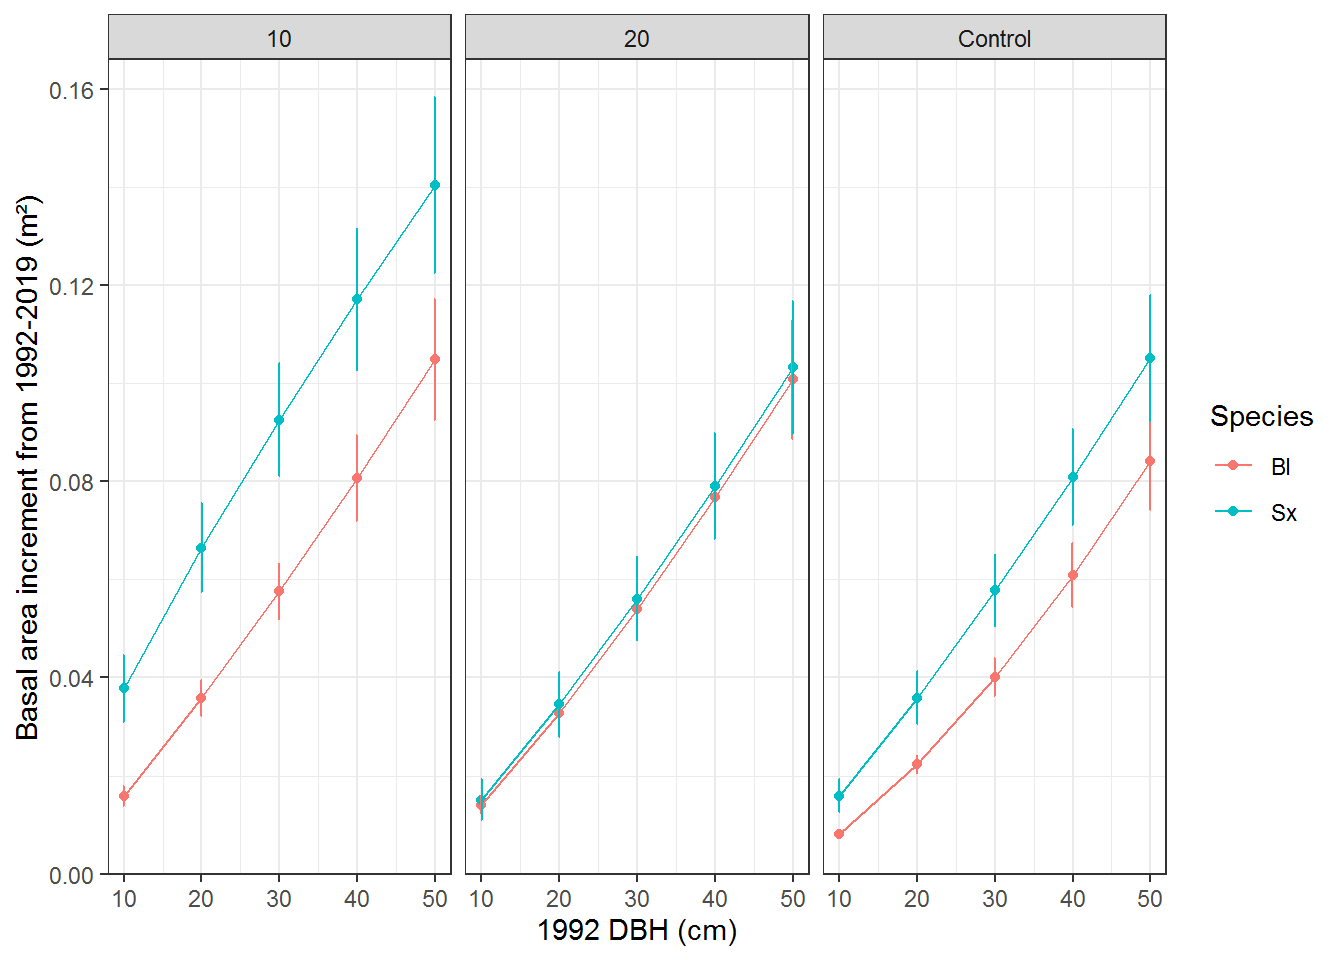
\includegraphics{_main_files/figure-latex/display tree growth figure-1.pdf}

Figure 1: Estimated marginal means of spruce and fir basal area increment (m²) across five inital DBH classes and three treatments. Whiskers are standard error of the mean. Responses are back-transformed from the model.

\begin{center}\rule{0.5\linewidth}{0.5pt}\end{center}

Appendix 6: Contrasts between predicted fir and spruce growth across treatment units and initial diameter classes. Ratio between predicted fir and growth is in `ratio' column.

\includegraphics[width=6.00in,height=4.00in,keepaspectratio]{_main_files/figure-latex/print fir spruce contrasts-1.png}

\begin{center}\rule{0.5\linewidth}{0.5pt}\end{center}

Appendix 7: Contrasts of predicted 1992-2019 tree growth among treatments within each species. Ratio of predicted growth between treatments is in `ratio' column.

\includegraphics[width=6.00in,height=7.75in,keepaspectratio]{_main_files/figure-latex/print treatment contrasts-1.png}

\begin{center}\rule{0.5\linewidth}{0.5pt}\end{center}

\hypertarget{stand-level-analyses}{%
\subsection{Stand-level analyses}\label{stand-level-analyses}}

\hypertarget{estimating-tree-height-from-diameter}{%
\subsubsection{Estimating tree height from diameter}\label{estimating-tree-height-from-diameter}}

Tree heights had a positive nonlinear relationship with diameter, for both species and across all time periods (Appendix 8). A comparison of height-diameter models showed that intercepts and slopes of log-transformed heights did not vary significantly (i.e., p\textgreater{}0.05) between species or time periods (not shown), therefore a single height-diameter linear mixed-effects model was developed using 870 tree height-diameter observations in the dataset, with log-transformed diameter as the fixed effect, and tree nested within plot as random effects. This model explained 86\% of variation in log-transformed heights, with an intercept of 0.256 and slope coefficient of 0.814 * log-transformed DBH (not shown). Residual and predicted vs actual height plots were assessed to ensure goodness of fit (Appendix 9). This model was applied to predict heights in trees without height measurements, and tree-volume estimates generated as per Nigh {[}-@nigh2016{]}.

\begin{longtable}[]{@{}l@{}}
\toprule
\endhead
\begin{minipage}[t]{0.39\columnwidth}\raggedright
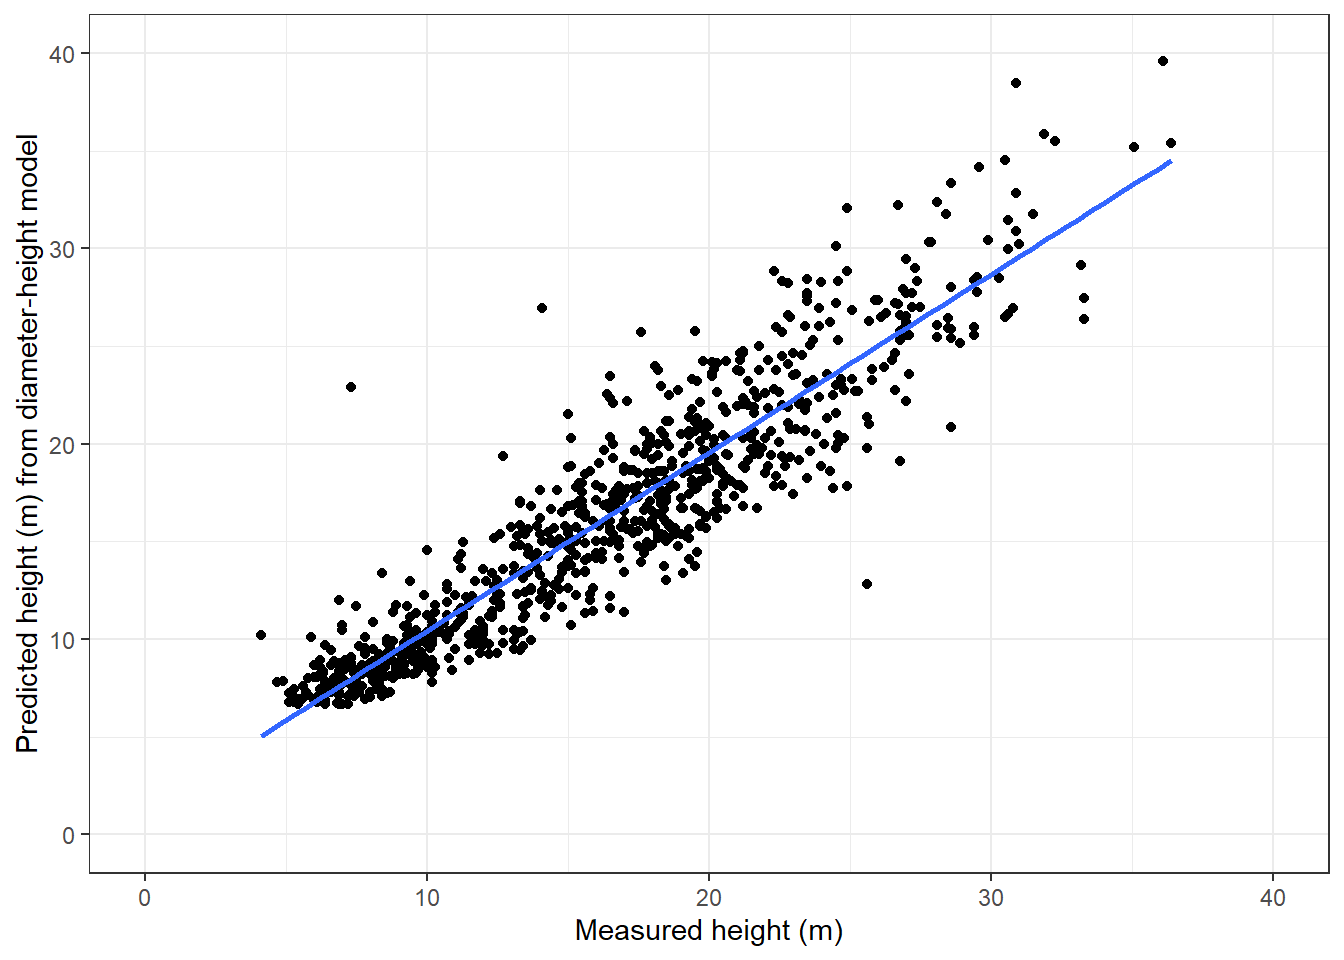
\includegraphics{_main_files/figure-latex/height model fit-1.pdf}\strut
\end{minipage}\tabularnewline
\bottomrule
\end{longtable}

Appendix 9: Scatterplot of predicted height(m) vs actual height(m) from diameter-height model.

\hypertarget{plot-means}{%
\subsubsection{Plot means}\label{plot-means}}

\emph{Observations:}

\begin{enumerate}
\def\labelenumi{\arabic{enumi}.}
\item
  All units increased volume, basal area and stand density over the 1992-2019 period (Figure 6).
\item
  The rate of change differed between units. The low RBA unit accrued basal area faster than the other two units over the 1992-2019 period, and this difference was significant (Appendix 10). The estimated rate of basal area increment in the low RBA unit was higher by by 8.4 and 7.8m² per hectare more than the high RBA and control units, respectively.
\item
  The low RBA unit also significantly increased its stand density by an estimated 340 stems per hectare more than the control unit. The rate of change in tree density did not differ significantly between the two harvested units.
\item
  The rate of change in volume in trees over 17.5cm DBH was barely significant between the two harvested units, and there were no significant differences between the control and harvested units.
\end{enumerate}

\begin{center}\rule{0.5\linewidth}{0.5pt}\end{center}

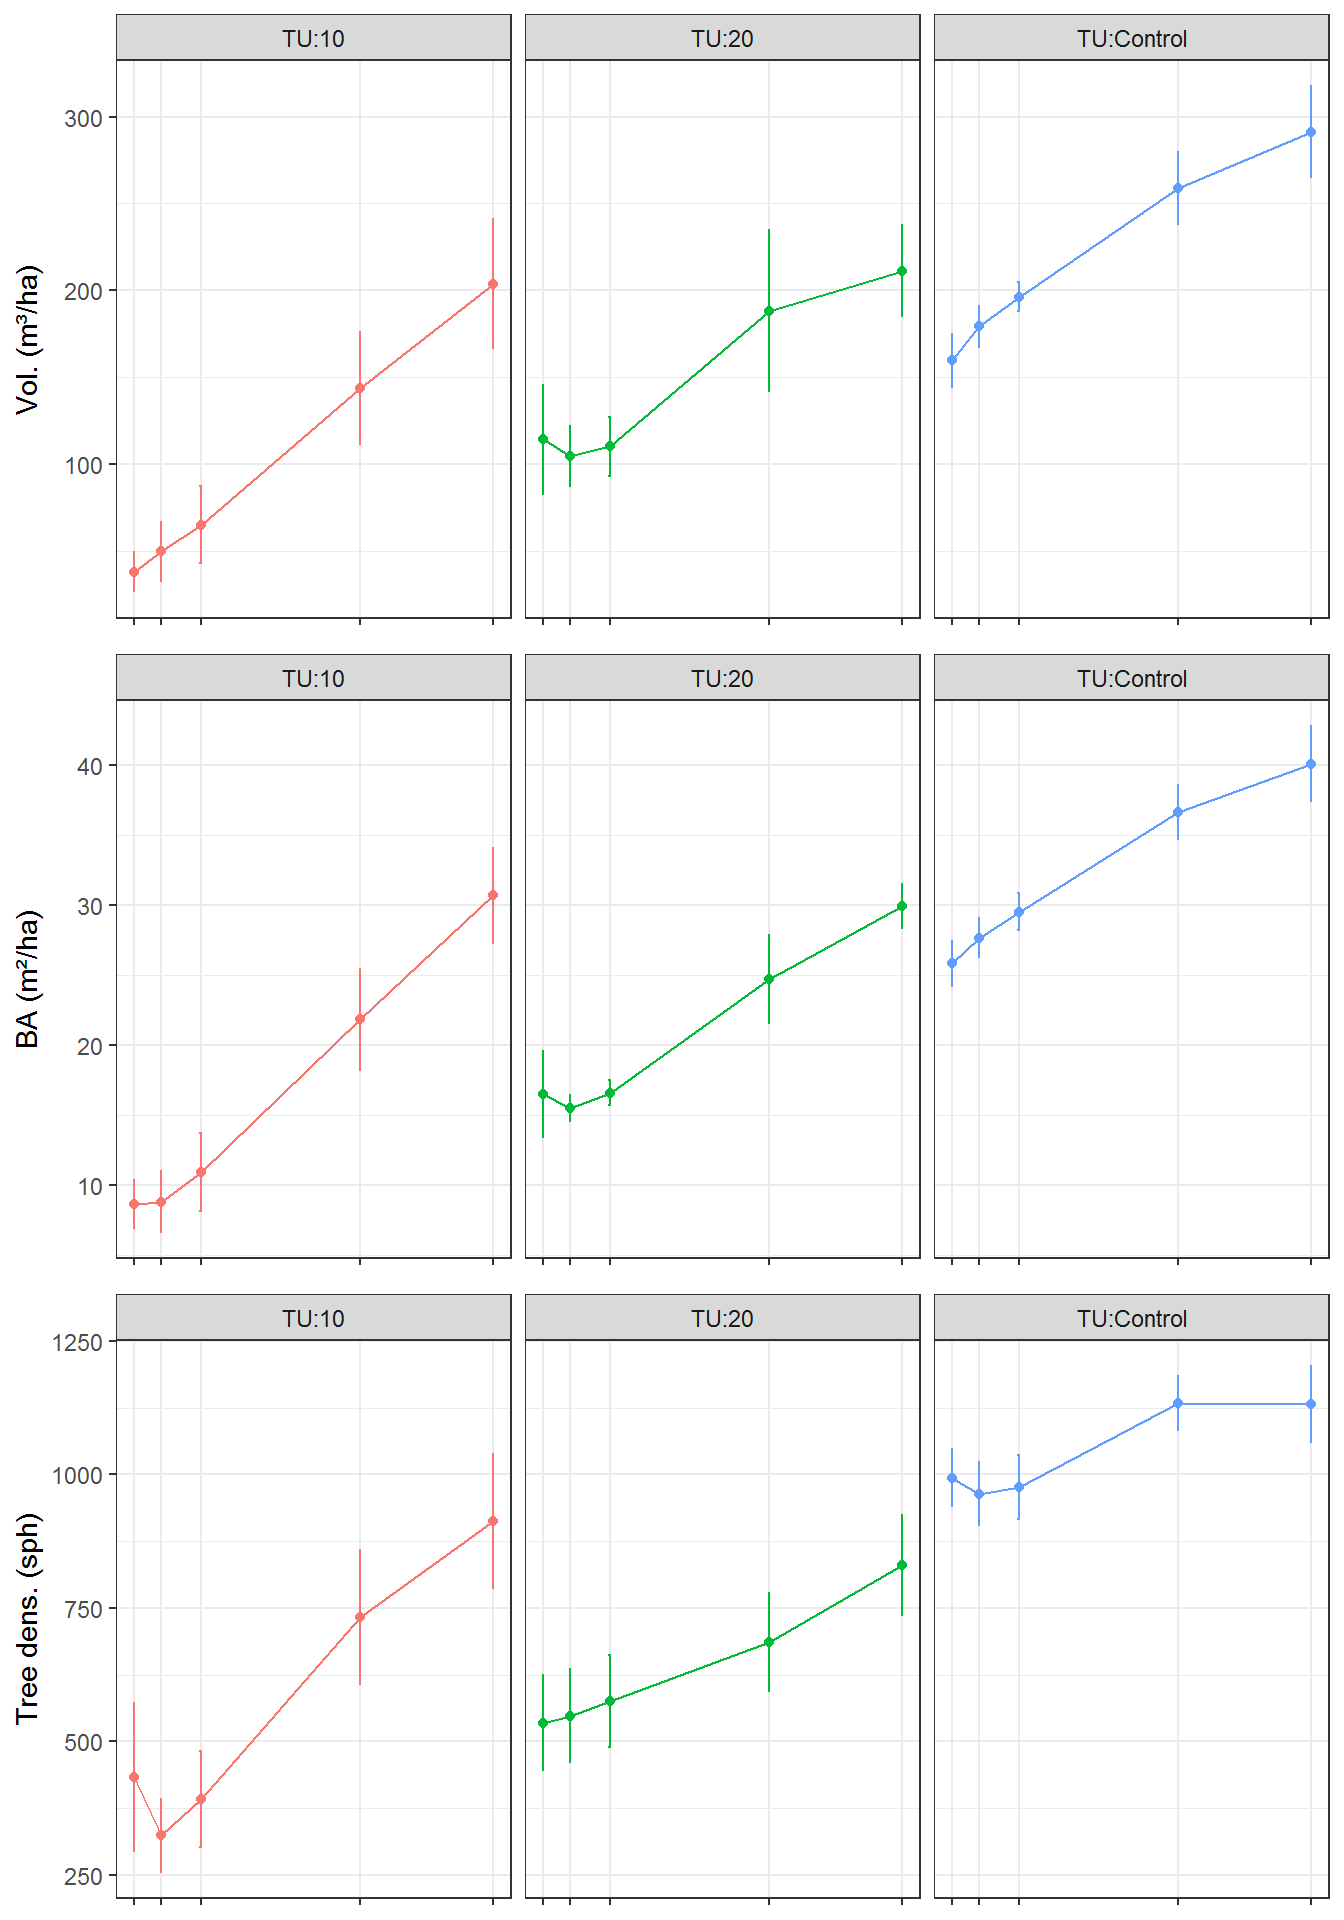
\includegraphics{_main_files/figure-latex/unnamed-chunk-1-1.pdf}

Figure 6: Mean plot attributes by treatment unit and year. Whiskers are one standard error of the mean. Vol., volume; BA, basal area; Tree dens., tree density; QMD, quadratic mean diameter

\emph{Note that sample size varies with year. Some plots were not measured in 1992. This likely explains the dip in basal area and volume in TU:20 from 1992 to 1994, despite no recorded mortality in 1992/1994.}

\begin{center}\rule{0.5\linewidth}{0.5pt}\end{center}

Table 2: Output from three separate linear models testing the effect of the interaction between treatment and year on plot-level volume, basal area and density.

\includegraphics[width=8.39in,height=2.92in,keepaspectratio]{_main_files/figure-latex/stand variable model output-1.png}
\emph{Trt, treatment; Sq., squares, Num., numerator; Den., denominator; DF, degrees of freedom}

\begin{center}\rule{0.5\linewidth}{0.5pt}\end{center}

Appendix 10: Contrasts of 1992-2019 stand structure development over 1992-2019 between treatments. Contrasts are shown for three variables: volume, basal area and stand density.

\includegraphics[width=6.74in,height=2.93in,keepaspectratio]{_main_files/figure-latex/show contrasts between plot means-1.png}

\hypertarget{stand-attribute-by-diameter-class}{%
\subsubsection{Stand attribute by diameter class}\label{stand-attribute-by-diameter-class}}

Among treatments and throughout the stand development after treatment, the stands have maintained a reverse-J diameter class distribution (Figure 4).\\
Immediately after the partial harvest, the diameter class distribution of volume differed between the treatment. In the 27 years since partial harvest, volume in all three treatment units was mostly concentrated in the 22.5-27.5cm DBH class, and mostly comprised of fir (Figure 2). Over both time periods shown in the figure and all three treatments, most of the spruce volume was concentrated in DBH classes spanning 37.5 to 47.5cm. Basal area trends were very similar to volume, and are not shown.

\begin{center}\rule{0.5\linewidth}{0.5pt}\end{center}

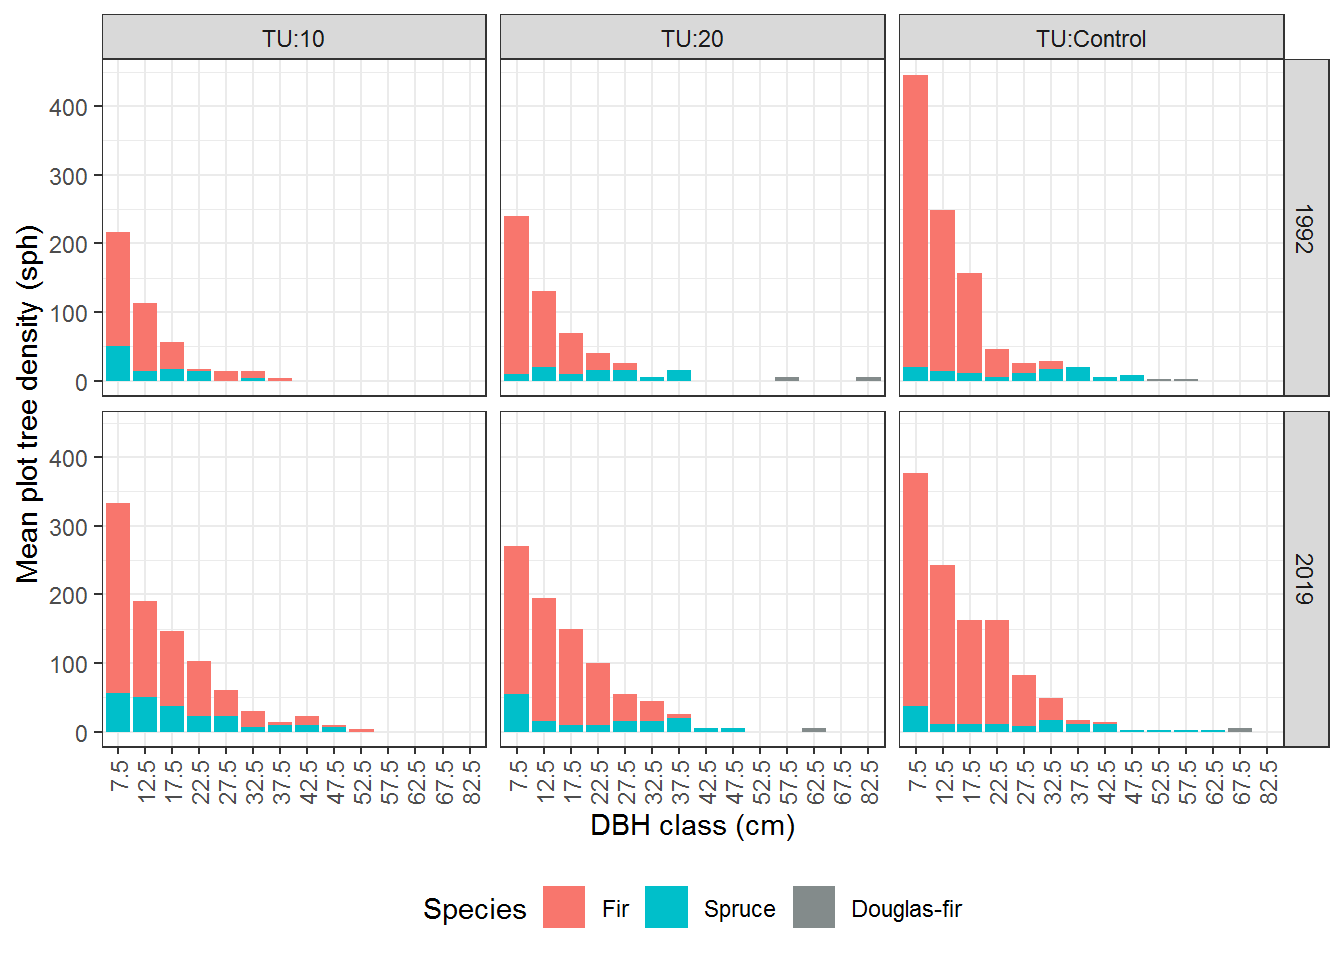
\includegraphics{_main_files/figure-latex/unnamed-chunk-2-1.pdf}

Figure 2: Mean plot volume distribution by diameter class and treatment, for two periods. Black line shows total volume. Volume calculated on trees meeting 17.5cm DBH limit. Spruce and fir contribution to volume by diameter class are shown with bar plots. Douglas-fir volume contribution by diameter class is not shown.

\begin{center}\rule{0.5\linewidth}{0.5pt}\end{center}

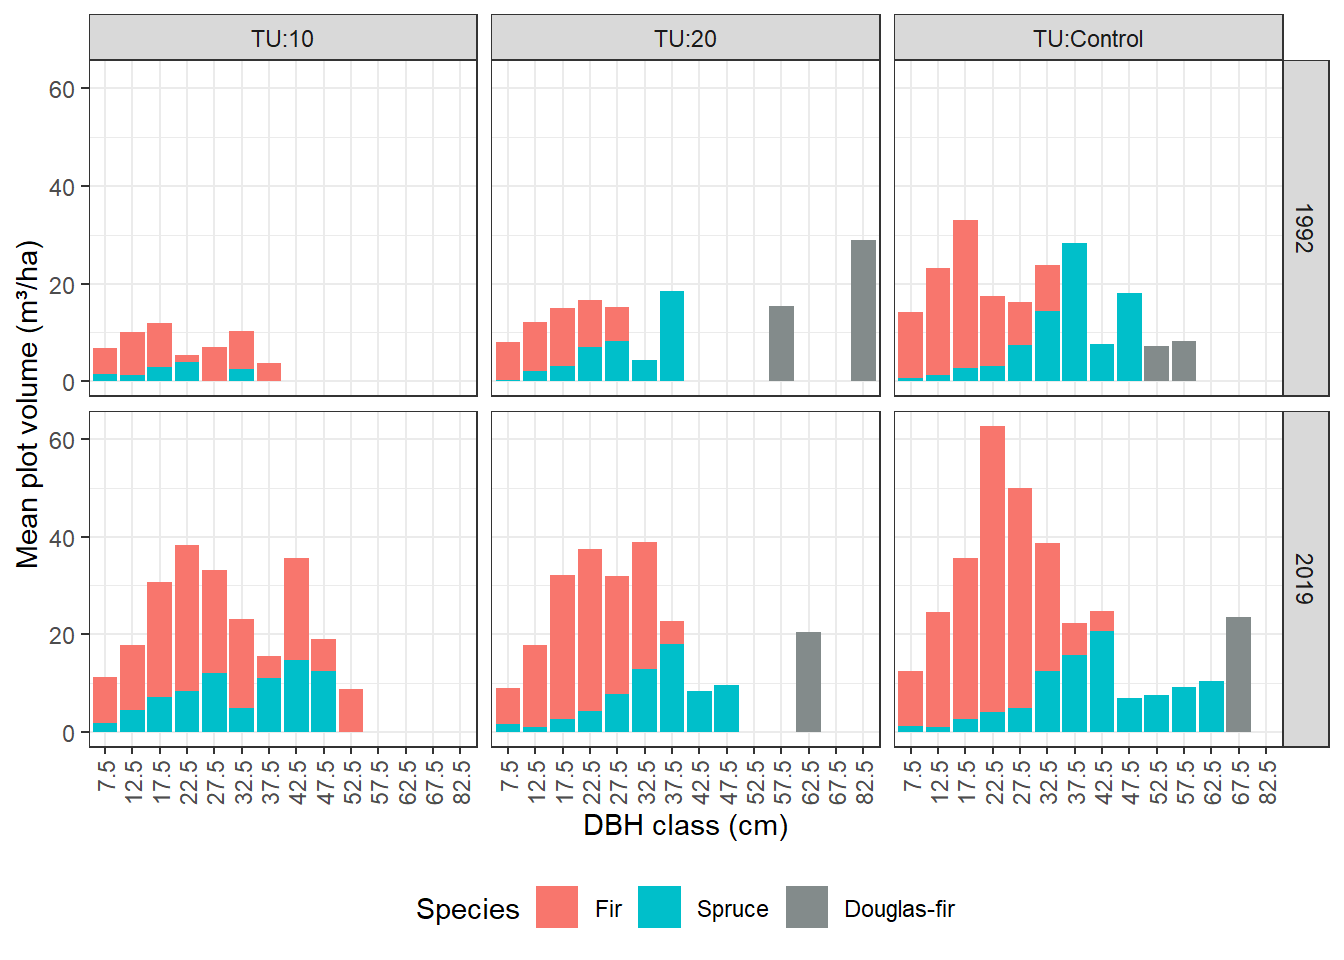
\includegraphics{_main_files/figure-latex/unnamed-chunk-3-1.pdf}

Figure 2: Mean plot volume distribution by diameter class and treatment, for two periods. Black line shows total volume. Volume calculated on trees meeting 17.5cm DBH limit. Spruce and fir contribution to volume by diameter class are shown with bar plots. Douglas-fir volume contribution by diameter class is not shown.

\emph{Note that in this figure, we show volume for all diameter classes. This is different than the stand-level estimate of volume, where we only estimate volume for trees that would be considered merchantable under conventional harvest in British Columbia (i.e., minimum 17.5cm DBH).}

\begin{center}\rule{0.5\linewidth}{0.5pt}\end{center}

\hypertarget{species-composition}{%
\subsubsection{Species composition}\label{species-composition}}

A comparison of proportional species composition by diameter class, treatment and year showed that fir and spruce were organized similarly between the high RBA and control units (Figure 8). In 1992, the largest diameter classes were dominated by spruce, whereas fir was the dominant species in the smallest diameter classes. This pattern was found for volume, basal area, and tree density. We only show volume in this document. By 2019, the fir-spruce composition by distribution class was maintained in these two units, with small increases in spruce composition in the smallest diameter class.

In the low RBA, the species composition distribution was different. Here, both species maintained a similar proportion of fir-leading across diameter classes smaller than 37.5cm DBH, whereas spruce formed the leading species in diameter classes above 37.5cm DBH, with the exception of the largest class.

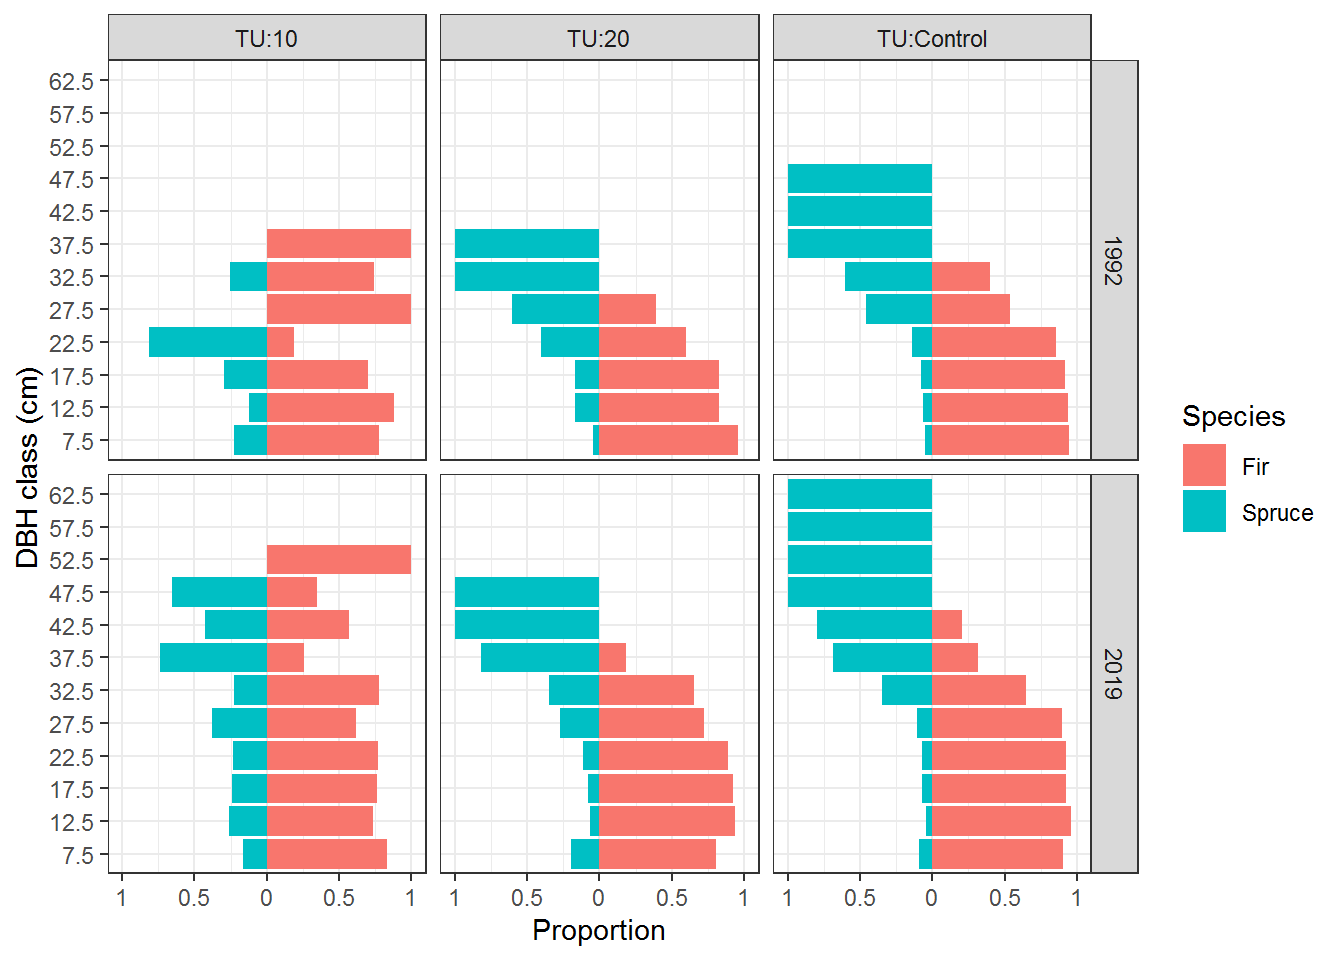
\includegraphics{_main_files/figure-latex/species composition plot-1.pdf}

Figure 8: Spruce-fir volume proportional composition by diameter class, treatment and year.

\emph{Note this figure is almost identical if we compare stems, basal area or volume. For brevity, we only show volume here.}

\hypertarget{mortality}{%
\section{Mortality}\label{mortality}}

A total of 95 trees (76 fir, 18 spruce, and 1 Douglas-fir) died from 1992 to 2019. No tree mortality was noted during the 1992 and 1994 data collection. By treatment unit, the control unit had the highest mortality, in terms of trees and basal area (
46.5 and
46.5\% of tree mortality, respectively). The high-removal treatment unit had the lowest mortality by number of trees and basal area (
12.1 and
12.1\% of tree mortality, respectively). Tree mortality was concentrated in the smaller diameter classes in the control and low-removal treatment unit, and most mortality occured during the most recent measurement period of 2009-2019 (
Figure 9).

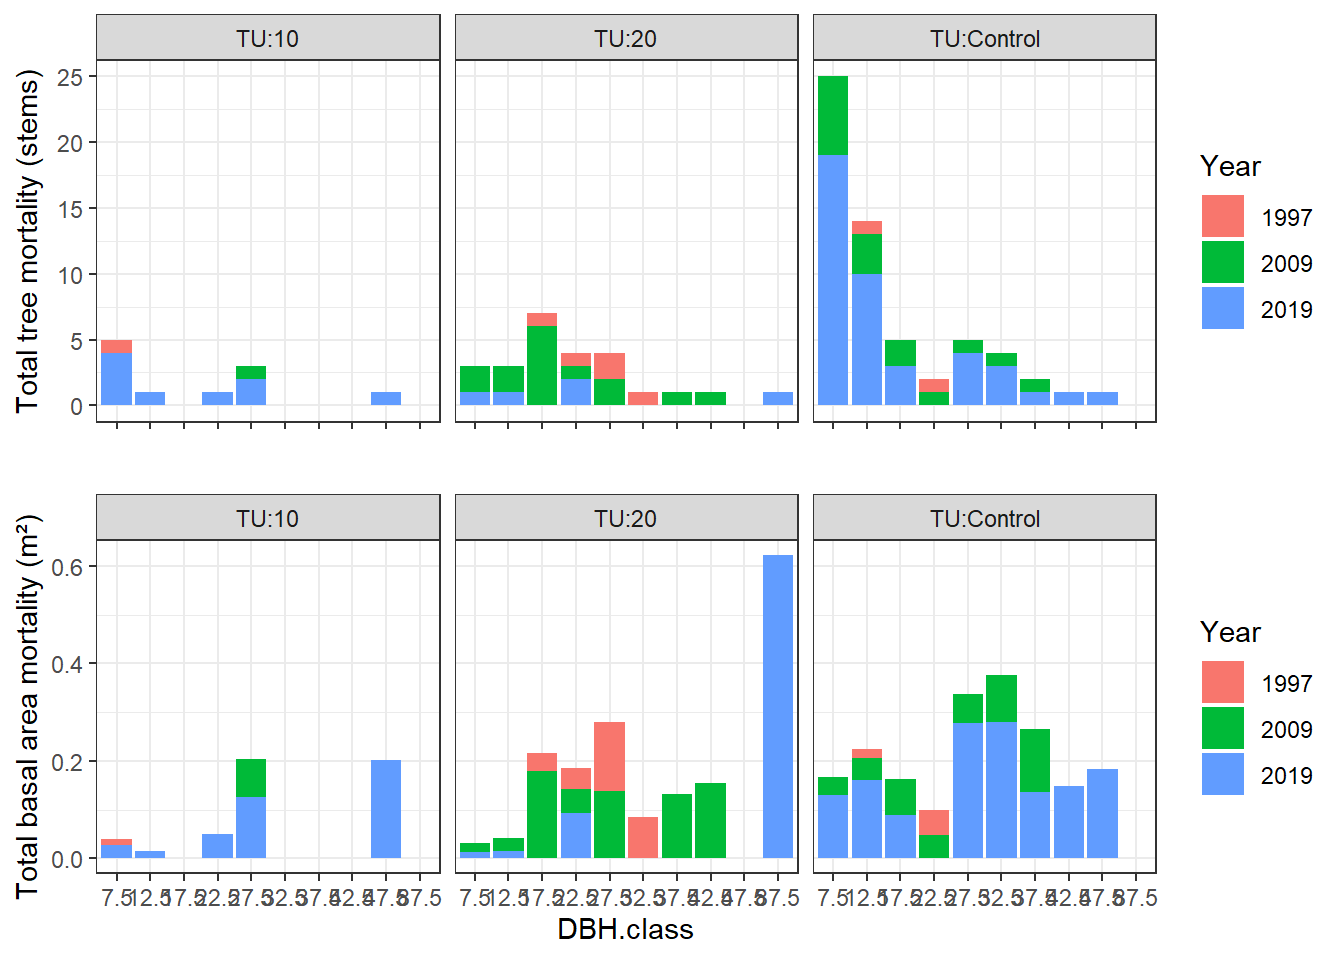
\includegraphics{_main_files/figure-latex/display mortality plot-1.pdf}

Figure 9: Total tree mortality recorded in plots from 1992-2019, presented as total stems (top panel) and basal area (bottom panel).

\begin{center}\rule{0.5\linewidth}{0.5pt}\end{center}

From Mike's email:
Eventually as BA stand density increases, density dependent mortality kicks in, because there is only so much growing space or access to site resources to go around. This can occur with the stand (conceptually or hypothetically) in two possible ways: (a) ``classic'' suppression of smaller tree classes through asymmetric competition of bigger trees shading out smaller ones, or (b) high stand densities suppressing the vigor of the whole stand through various means, suggesting more symmetric competition -- i.e.~the idea that small trees compete for growing space with big ones as well. Asymmetric competition is generally accepted by most foresters and silviculturists; symmetric competition less so, and is often harder to demonstrate.

\emph{For the discussion: it seems that we're seeing mortality increasing in the plots, especially the control unit over the last 11 years. Does this reflect the density-dependent mortality that Mike refers to above?.}

More from Mike on mortality:

The thing about unevenaged or complex stand management, esp in `wilder' BC stands, is that we are working in stands with a long legacy of pre-existing ecosystem processes before we enter the stand to manipulate them. Clearcutting liquidates these legacies for the most part, and traditional silviculture and GY has not had to deal with mortality much, other than clearly density dependent suppression of smaller dbh classes. {[}Side issue: most BC experience and data with unevenaged stands has been in IDF, which have been fire excluded on dry sites, and unevenaged structures allowed to develop. We must be careful about comparing Summit data to IDF precedents, because of substantial differences in ecology.{]}

And we are working a more extensive level of management in the SBS and ESSF, where our stands are older, and not manicured nor vacuumed up for mortality and blowdown. From an ecosystem management point of view, that Is probably a good thing.

So warts and all, I think mortality is an inherent characteristic of the types of spruce-balsam stands and management we are studying. Expecting and documenting mortality was built into the EP 1162 working plan. The treatment effects we anticipate are the net stand growth = gross growth minus mortality.

Conceptually, tree mortality following the 1991/92 harvest (and subsequent sanitation felling) functions as a BA removal from the live-tree pool. In most plots, BA of trees that die within a measurement period is subsumed or overridden by the total BA growth of the rest of the trees during that period.

Where the periodic data trends get messier is where single big trees or a cluster of trees gets killed by something, resulting in a pulse of BA mortality. Examples: The great big Fdi in Plot 18, or notably, about 3-4 big Sx in Plot 3 that got nailed by spruce beetle.

In our results and discussion:
1. We can report on what stand growth and development trends seem to be clearly and unambiguously influenced by initial BA conditions, and the magnitude of these treatment effects.
2. A component of tree mortality (e.g.~certain size classes) may be density dependent.
3. A component of tree mortality may be density-independent (a.k.a stochastic or chaotic).
4. By reporting on all the above, we are providing managers with results that integrate silvicultural expectations observations from real-life ``messy'' stands which will experience all of the above. By keeping our eye on overall stand growth and performance following treatment, we can inform / reassure managers that individual tree mortality events are not the end of the world, but rather need to be viewed in the context of overall stand dynamics and growth expectations.

\hypertarget{miscellaneous}{%
\section{Miscellaneous}\label{miscellaneous}}

Miscellaneous figure, data and ideas that don't have a home yet.

\hypertarget{plot-level-figures}{%
\subsection{Plot-level figures}\label{plot-level-figures}}

Below are some plot-level figures just to examine the data and look for outliers.

\hypertarget{volume}{%
\subsubsection{Volume}\label{volume}}

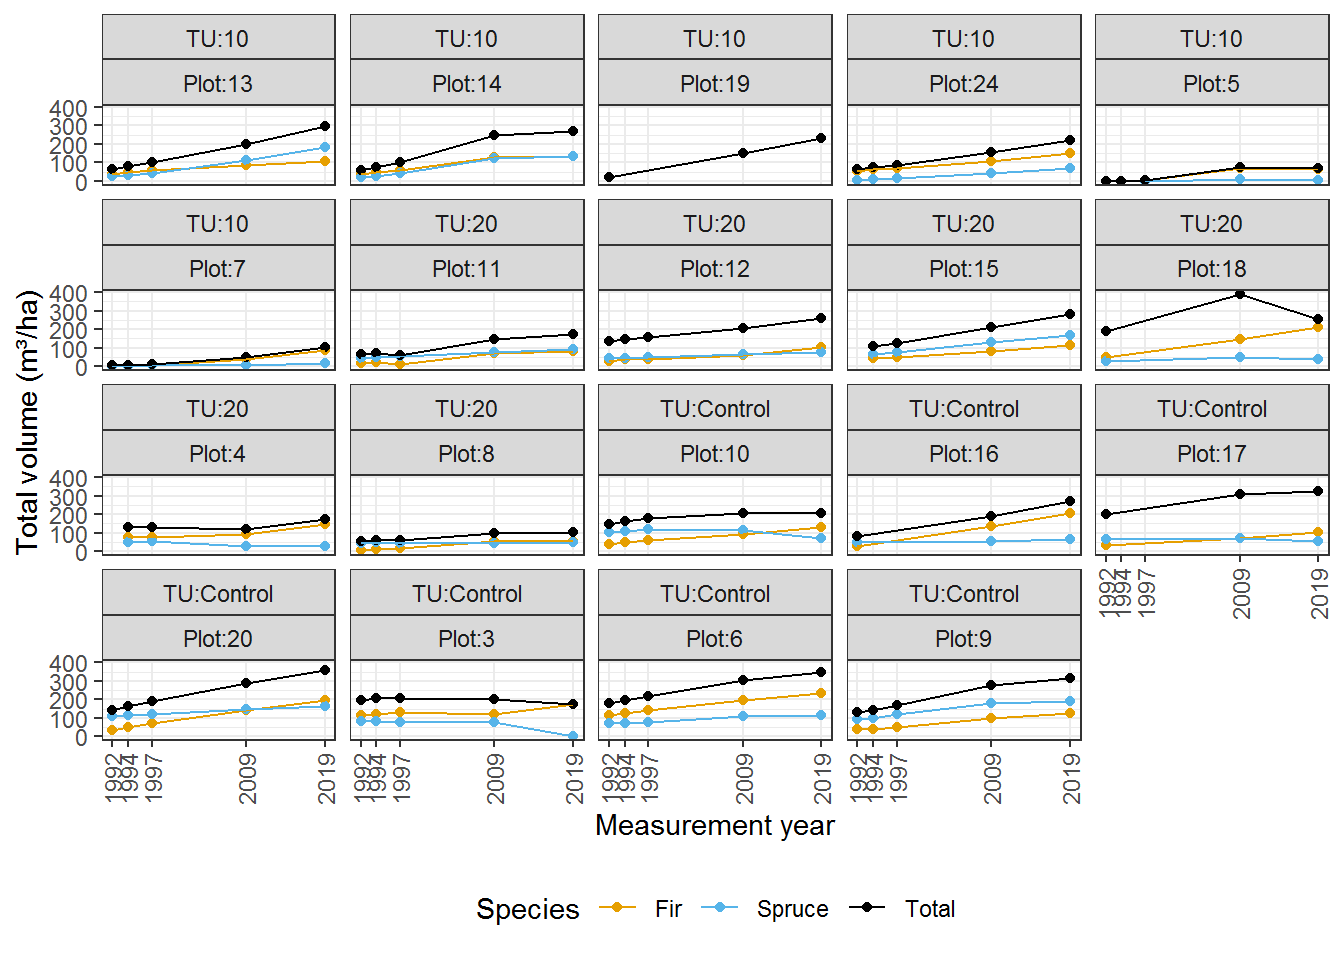
\includegraphics{_main_files/figure-latex/stand volume plot-1.pdf}

\hypertarget{quadratic-mean-diameter}{%
\subsubsection{Quadratic mean diameter}\label{quadratic-mean-diameter}}

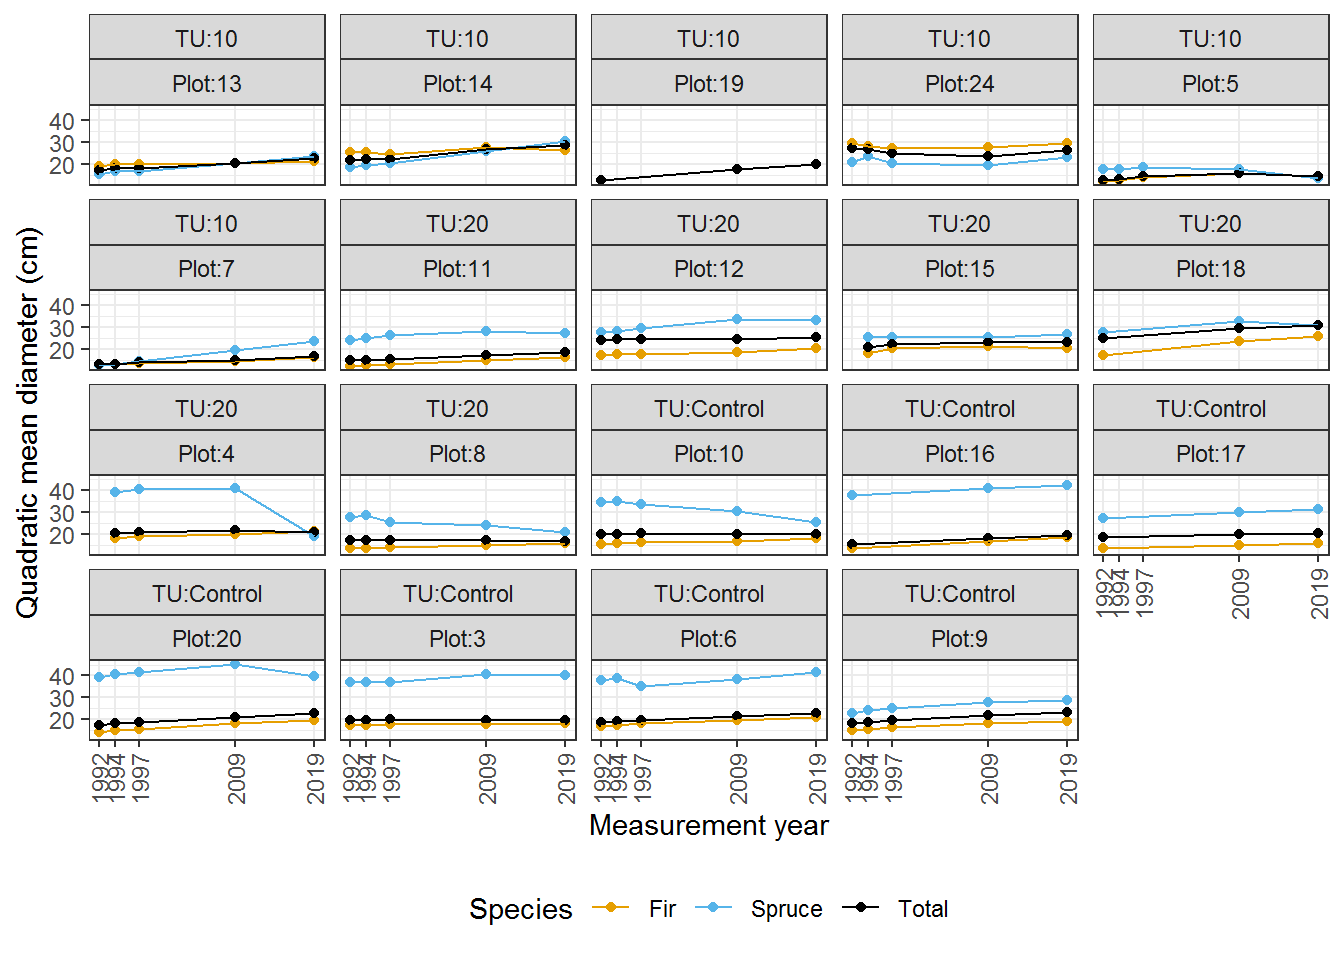
\includegraphics{_main_files/figure-latex/QMD plot-1.pdf}

From Mike's e-mail:
QMD is traditionally or commonly used as a comparative stand parameter in more even-aged stands like plantations or even-aged thinning trials. Trees grow and BA increases, but numbers of live trees do not increase, they only decrease through suppression or harvesting. Usually no recruitment. QMD and its variants are often the root of various stand density indexes, and these SDI's usually are not used or designed for complex stands with more recruitment or multiple stand layers. Mensurationists often love QMD and SDI as they are mathematically elegant, and in even-aged structures, can be very useful management tools. I am generalizing regarding the literature and stand mgmt. practices, but that basically true overall.

Your QMD graphs are very interesting. Within individual plots, BA tends to increase progressively most of the time, except when a major disturbance or death(s) of really large trees occur. However, the flow of smaller trees being recruited in some stand conditions at Summit increases sph over time, and drives down QMD over time in these situations.

Over the full spectrum of stand conditions at Summit, where the stand structure is complex and generally unevenaged, the QMD trend is dynamic over time. At lower densities with more stem recruitment, it will tend to decrease over time even though individual trees are growing in diameter quickly, because sph is increasing rapidly. At middling BA densities, QMD may be relatively stable, as recruitment moderates or slows, and individual trees still grow steadily. However, as stands get denser in BA over time, and trees get older and slower growing, eventually climatic events (e.g.~wind or snow damage) or biotic events (stem rots or beetles) will increase the likelihood that moderate-sized to larger trees will succumb to various types of mortality. This mortality could be fairly predictable (e.g.~big Sx succumbing to beetle above a certain size) or chaotic (such as stand damage to snow and wind). So, conceptually QMD reaches its maximum at some point, and then QMD will decrease or plummet as the stand starts to get gappy and undergo understory recruitment.

Overall, QMD tends to be maximized at the point in stand development where the most growth is accumulated on the fewest live trees spread over the area. Definitely an oft-desired optimum end-point for traditional timber managers, at which point they would want to harvest. But QMD is not the be-all and end-all if alternative stand structures and stand management objectives are favored.

Our monitoring plot size (0.05 ha) will not capture all of the within-stand variability of more chaotic disturbances.

\end{document}
